\documentclass[11pt]{article}


\usepackage{arxiv}
\usepackage{subfig}
\usepackage[utf8]{inputenc} % allow utf-8 input
\usepackage[T1]{fontenc}    % use 8-bit T1 fonts
\usepackage{hyperref}       % hyperlinks
\usepackage{url}            % simple URL typesetting
\usepackage{booktabs}       % professional-quality tables
\usepackage{amsfonts}       % blackboard math symbols
\usepackage{nicefrac}       % compact symbols for 1/2, etc.
\usepackage{microtype}      % microtypography
\usepackage{lipsum}
\usepackage[title]{appendix}
\usepackage{graphicx}
\usepackage{caption}
\usepackage{graphics}
\usepackage{multirow}
\usepackage{float}
%\usepackage{vmargin}
\usepackage[a4paper, inner=1cm, outer=1cm, top=1cm,bottom=1cm, bindingoffset=0.4cm]{geometry}

%\captionsetup[table]{skip=10pt}


%\setmarginsrb{2 cm}{2 cm}{2 cm}{2 cm}{2 cm}{2 cm}{2 cm}{2 cm}
\title{COMP6208: Advanced Machine Learning}


\makeatletter
\def\thickhline{%
  \noalign{\ifnum0=`}\fi\hrule \@height \thickarrayrulewidth \futurelet
  \reserved@a\@xthickhline}
\def\@xthickhline{\ifx\reserved@a\thickhline
              \vskip\doublerulesep
              \vskip-\thickarrayrulewidth
             \fi
      \ifnum0=`{\fi}}
\makeatother

\newlength{\thickarrayrulewidth}
\setlength{\thickarrayrulewidth}{2\arrayrulewidth}

\author{
  Brent De Hauwere$^1$, Matthew De Vries$^2$, Dimitris Mallios$^3$, Ilias Kazantzidis$^4$ \\
  %University of Southampton\\
  \texttt{$^1$bdh1g19, $^2$mrdv1n19, $^3$dm1n19, $^4$ik3n19}
  %\textit{*All authors contributed equally to the writing and research in this study. Their names are listed in alphabetical order.}
}

\begin{document}
\maketitle

% \vspace{-1cm}
\vspace{-1.2cm}
\section{Introduction}
Electrocardiogram (ECG) analysis has been established at the core of cardiovascular pathology diagnosis since its development in the twentieth century \cite{alfras}. The main problem with manual analysis of ECG signals, similar to many other time-series data, lies in difficulty of detecting and categorizing different waveforms and morphologies in the signal. For a human, this task is both extensively time-consuming and prone to errors \cite{Kachuee_2018}. 

\vspace{-0.3cm}

\section{Data}
This dataset is composed of heartbeat signals derived from the famous dataset in heartbeat classification, the MIT-BIH Arrhythmia Dataset. The number of samples is large enough for training a deep neural network as well as using other advanced methods in machine learning. The dataset is described:
\begin{itemize}
    \item Number of Samples: 109446
    \item Number of Categories: 5
    \item Sampling Frequency: 125Hz
    \item Data Source: Physionet's MIT-BIH Arrhythmia Dataset
    \item Classes: ['N': 0, 'S': 1, 'V': 2, 'F': 3, 'Q': 4]
\end{itemize}

This dataset has been used in exploring heartbeat classification using deep neural network architectures, and observing some of the capabilities of transfer learning on it. The signals correspond to electrocardiogram (ECG) shapes of heartbeats for the normal case and the cases affected by different arrhythmias and myocardial infarction. 

\begin{figure}[h]
    \centering
    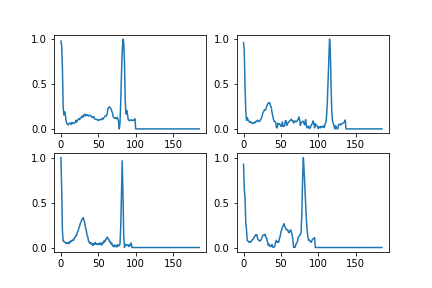
\includegraphics[width=0.5\textwidth]{images/heartbeats.png}
    \caption{Examples of the data}
    \label{fig:examples}
\end{figure}

\section{Reasons}
We chose this dataset due to the intriguing, challenging and useful aspect of medical topics and especially the ones concerned with the heart. A slight improvement in the real-time recognition of an abnormal heartbeat by an implanted device to a patient's heart could be crucial for them. We are not used to working with time series or signal data and this presents a challenge. Moreover, the specific dataset will give us the chance to apply both baseline traditional techniques and state-of-the-art deep learning approaches (LSTM, CNN, etc) in order to potentially demonstrate the superiority of the later in large datasets like this. We also hope that transfer learning and other advanced techniques will prove beneficial. We expect many challenges with preprocessing but none that we will shy from.

\nocite{*}

\bibliographystyle{plain}
\bibliography{biblist}
\end{document}

